\section{Versuchsaufbau}
\subsection{Aufbau des Pendels}
Eine Skizze des Versuchsaufbaus ist auf Seite 
\pageref{pic:skizze_versuchsaufbau} im Anhang zu finden.
Für ein Doppelpendel, das auch Überschläge des unteren Pendelglieds erlaubt, mussten die Verbindungen der Pendelmassen als Stäbe gebaut werden. Dabei galt es zu beachten, dass ein möglichst geringer Teil der Gesamtmasse in den Pendelstäben liegt. Die Wahl des Materials fiel auf Acryl, da es bei relativ geringem Gewicht die erforderliche Steifigkeit liefern kann. Das obere Pendelglied wurde symmetrisch auf beiden Seiten des Pendels gebaut um Kräfte zu vermeiden, die Schwingungen außerhalb der gewünschten Ebene verursacht hätten. Für den unteren Stab wurde eine Materialstärke von $5 mm$ gewählt, für den oberen Stab, war aufgrund der doppelten Ausführung eine Stärke von $3 mm$ ausreichend.
%(Genaue Maße der Platte siehe Abb. \ref{})
Auch diese dünne Materialstärke liefert ein Gewicht von $70  g$ pro Stab konnte aber aufgrund der Anforderungen an die Steifigkeit und Kosteneffizienz nicht unterschritten werden.\\
%70 g obere Platte

Um ein möglichst einfaches Modell zu erhalten, wurde versucht, die Reibung in den Achsen des Pendels zu minimieren. Die Lagerung wurde durch Kugellager der Firma FAG realisiert. Es wurden zwei Lager in der Aufhängung des Pendels integriert sowie ein weiteres Kugellager in der oberen Masse.
Die Gewindestange, das Kugellager sowie die sechs Schrauben und Muttern der oberen Masse kommen zu einer Masse $ m_1$ von $301 g$ zusammen. Um das Modell zu vereinfachen wurde versucht, eine möglichst gleiche Masse für $ m_2 $ zu finden. Hier kam ein Gewicht aus dem Lager des Projektpraktikums mit einer Masse von $297 g$ zum Einsatz.

\subsection{Messung der Pendelbewegung}
Um den Aufenthaltsort der Massen in der Pendelebene mit einem geringen zeitlichen Intervall aufzunehmen wurde eine Kamera eingesetzt. Um nach dem Versuch die X, Y Daten in einer Tabelle zu erhalten, wurde die Videotracking Software \enquote{Tracker} von Open Source Physics \footnote{http://www.cabrillo.edu/~dbrown/tracker/} eingesetzt.
Bei Testaufnahmen stellte sich heraus, dass das Programm dazu neigte, sofern kein optimaler Kontrast des Objekts zum Hintergrund herrschte, in einigen Frames Punkte im Hintergrund statt dem Objekt zu fokussieren. Als eine Weitere Hürde stellte sich die Bewegungsunschärfe dar, besonders in Phasen mit hoher Geschwindigkeit verschwamm der Trackingpunkt mehr zu einer Linie, die die Software dann nicht mehr zuordnen kann. Um einen hohen Kontrast zum Hintergrund zu erhalten, wurden die Massen mit LED markiert und der Versuch wurde in einem sonst dunklen Raum durchgeführt. Um die Bewegungsunschärfe zu minimieren wurde eine Kamera mit möglichst geringer Minimalverschlusszeit bei gleichzeitig guter Lichtausbeute gesucht. Diese Anforderungen konnten von einer Spiegelreflexkamera mit Videomodus erreicht werden. Auf den Einzelbildern des Videos erschienen die Marker des Pendels bei einer Verschlusszeit von $\frac{1}{2000} s$ zu allen Zeiten als Punkte.
\ref{foto-kamera}
\begin{figure}
\centering
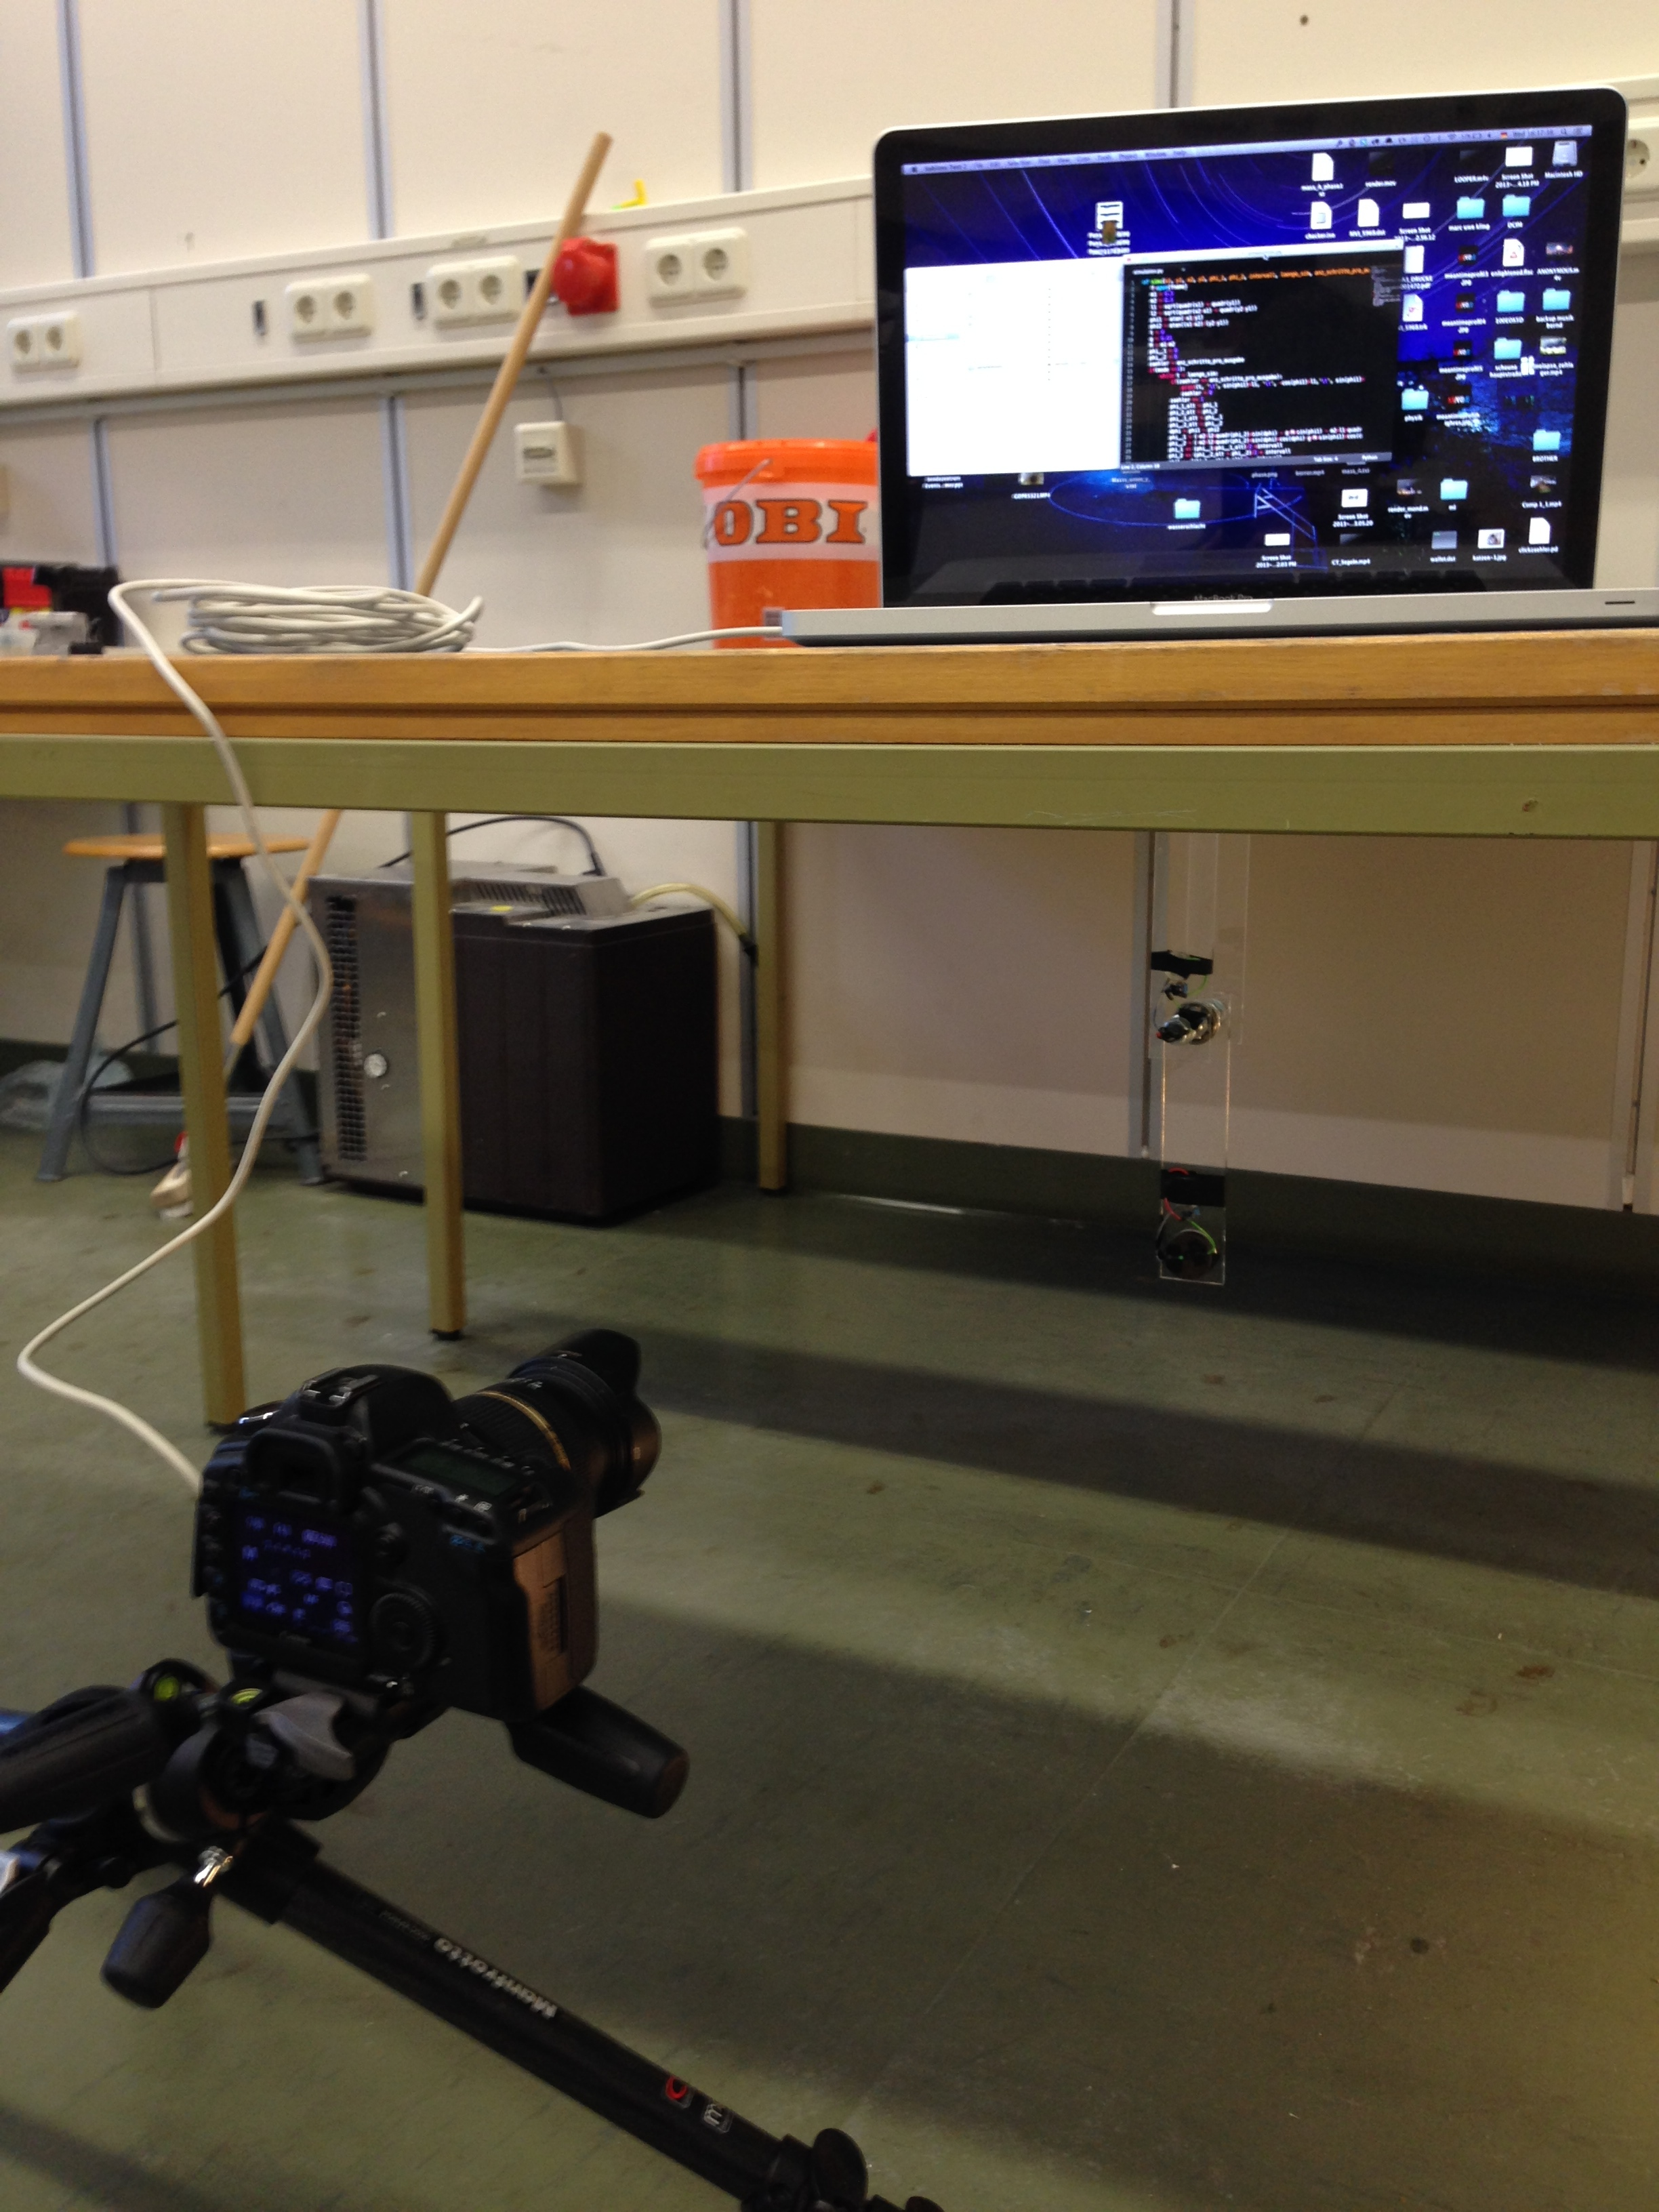
\includegraphics[width=.4\textwidth]{images/kamera}
\caption{Versuchsaufbau mit Kamera}
\label{photo-kamera}
\end{figure}
\begin{figure}
\centering
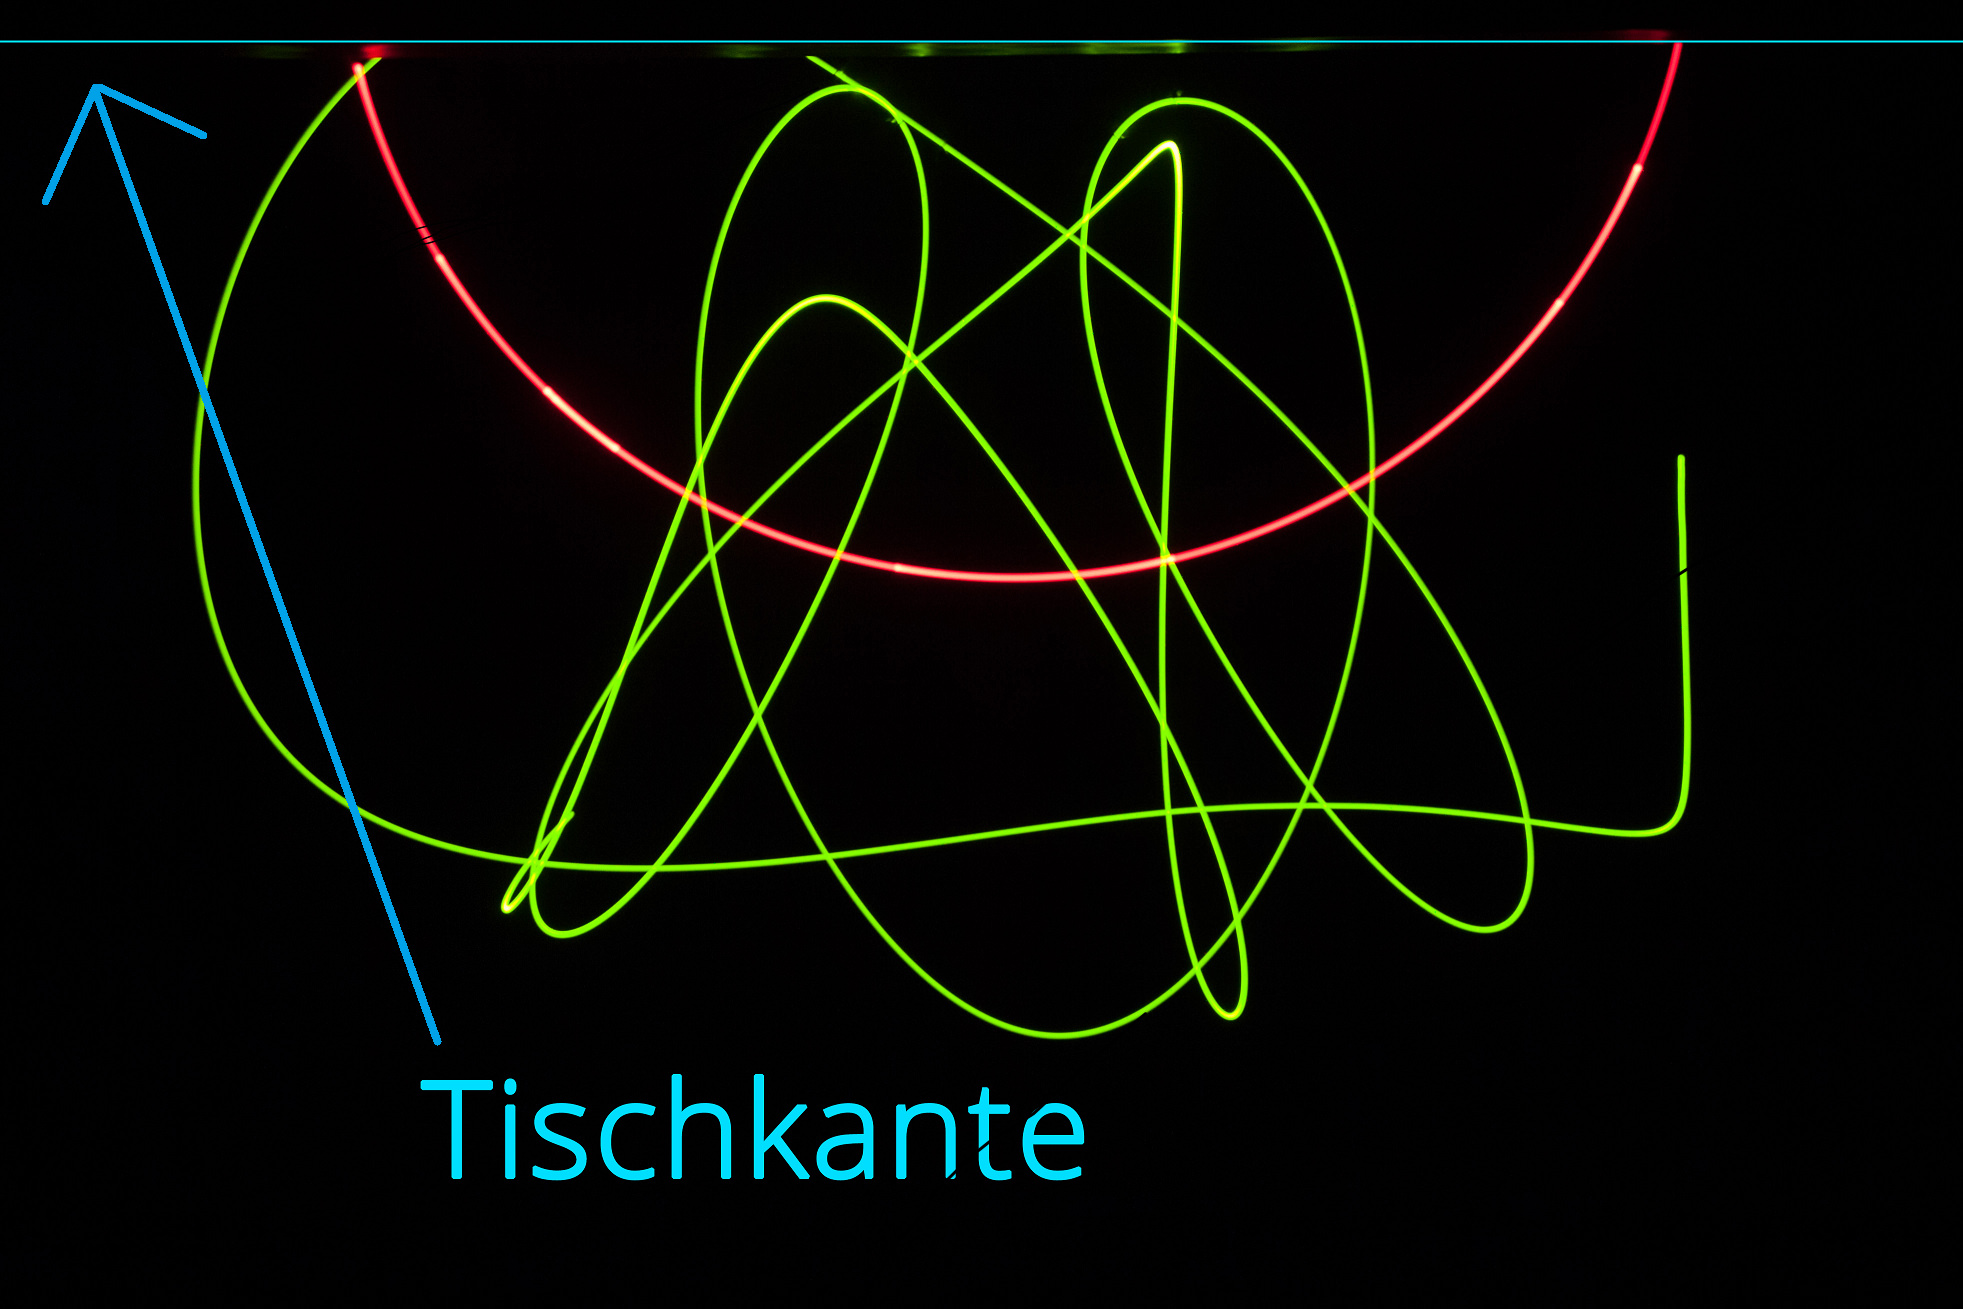
\includegraphics[width=.7\textwidth]{images/tischkante.jpg}
\caption{Tischkante verdeckt LED}
\label{tischkante}
\end{figure}
 Die Punkte ließen sich im Allgemeinen gut durch die Video Tracking Software analysieren, abgesehen von Spezialfällen in denen sich eine der Massen über der Tischkante und damit außerhalb des für die Kamera sichtbaren Bereichs befand.(siehe \aref{tischkante})
Als Nachteil der Spiegelreflexkamera kann gesehen werden, dass eine Aufnahme von 30 Bilder pro Sekunde die maximale Framerate der Kamera darstellt.
\begin{comment}
\begin{figure}
\includegraphics[scale=1]{images/platten}
\end{figure}
\end{comment}